


La figure \ref{transformationimage} nous montre un exemple de transformation d'une image de maison réalisé en 2 traits de crayons. 

\begin{figure}[h]
	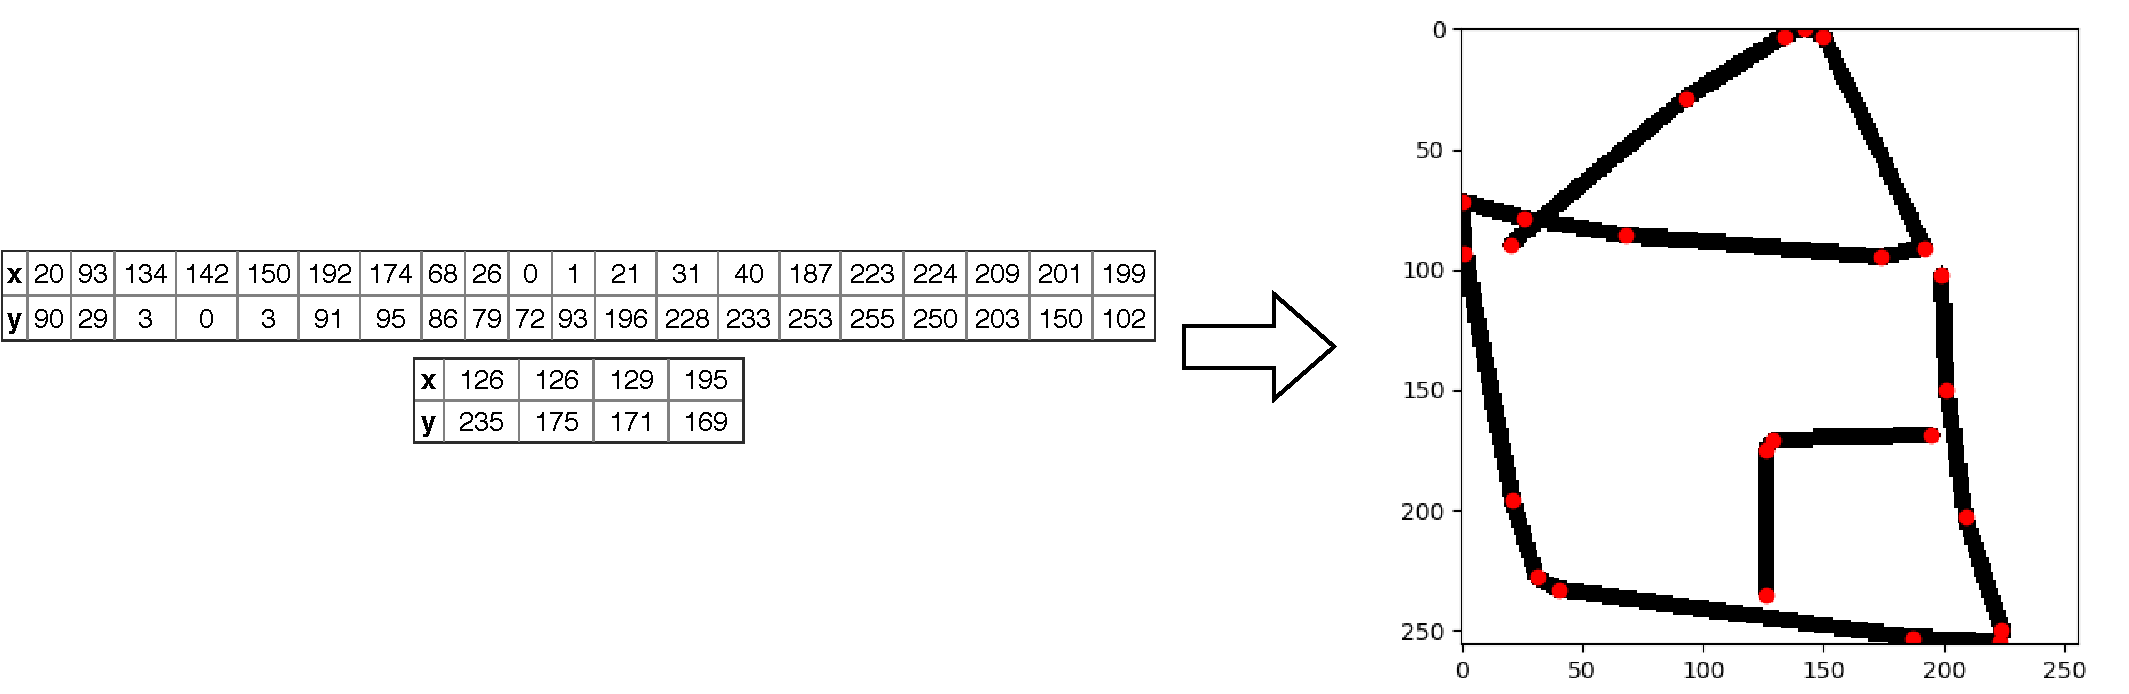
\includegraphics[width=\linewidth]{images/Transformations_horizontal.pdf} % Figure image
	\caption{Transformation de vecteur à image} % Figure caption
	\label{transformationimage} 
\end{figure}

La plupart des images sont loin d'être facile à apprendre pour un ordinateur, puisque que ces données ne sont pas filtrées par un humain qui peut valider si l'image est bonne. N'importe quel individu peut contribuer à cette base de données. Pour cette raison, on peut observer des images qui peuvent varier énormément pour une même classe. La figures \ref{frogs} nous permet de voir différentes images pour la classe \emph{frog}.



\begin{figure}[h]
	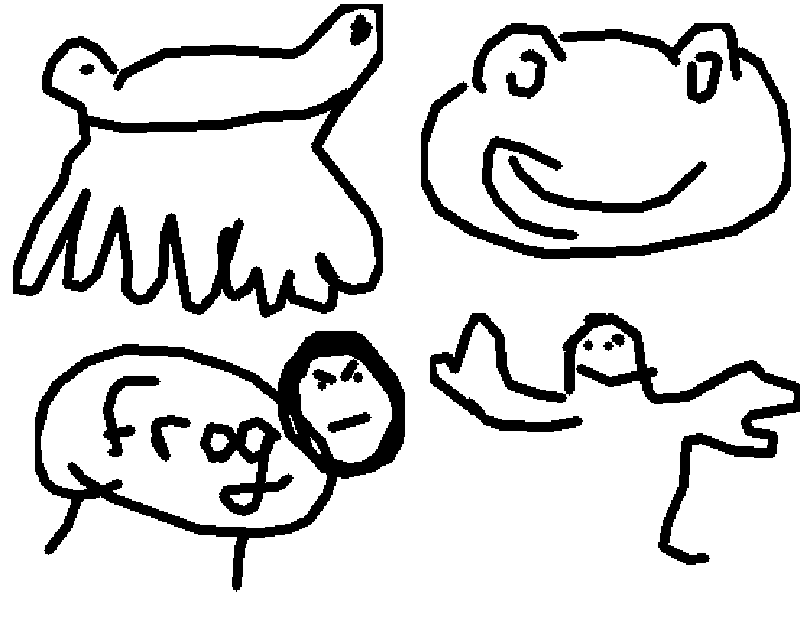
\includegraphics[width=\linewidth]{images/Combo_frogs.png} % Figure image
	\caption{Différentes images de la classe frog} % Figure caption
	\label{frogs} 
\end{figure}


On peut voir que les utilisateurs n'adoptent pas tous les mêmes techniques pour dessiner un même objet. Également puisque les utilisateurs ont seulement 20 secondes pour faire leur dessin, certains d'entre eux sont parfois incomplets. Comme aucun filtrage n'a été fait, on peut constater également que certaines images ne sont pas réalisés dans le but exact du projet (certains utilisateurs ne dessinent pas la bonne catégorie ou bien ne font qu'écrire le nom de la classe)
